\documentclass{../src/bcthesispart}
\title{Base games}
\author{Bas Cornelissen}
\begin{document}

%——————————————————————————————————————————————————————————

\appendixtitle{Base games}%
	{Base games}%
	{counting-games}{%
	%
	% Abstract
	% ————————
	This appendix mathematically derives the implicit biases in the additive naming game and presents some further analyses of the parameters of the game.
}

%——————————————————————————————————————————————————————————



%——————————————————————————————————————————————————————————
\subsection{Implicit biases in the additive naming game}

The additive base game strongly favours the use of the highest base.
To quantify that bias, we ask what the probability is that an agent, without any past experience, will use a certain base in the next round.
‘Without past experience’ is important, since we are interested in the \emph{bias}, similar to the Bayesian naming game.
The problem, I think, becomes much more intuitive if you keep the following diagram in mind:





%- - - - - - -
\begin{figure}[h!]
	\centering
	%\documentclass{../src/bcthesispart}
%\begin{document}

\begin{tikzpicture}[yscale=.5,xscale=1]\sffamily\footnotesize

	% Axis with numbers
	\def\axisy{-1.5}
	\foreach \x in {0,...,9} {
		\pgfmathsetmacro{\n}{int(11 + \x)}
		\node at (\x, \axisy-.7) {$\n$};
		
		\draw[dotted] (\x, 4) -- (\x, \axisy);
	}	
	\draw[line width=1] (0,\axisy) -- (9,\axisy);
	\foreach \x in {0,...,9}{
		\draw (\x, \axisy-.15) -- (\x, \axisy+.15);
	}
	\node at (-1,\axisy-.7) {$\mathcal{N}$};

	% x labels for E^{-1}(X)
	\foreach \x in {0,...,4} {
		\pgfmathsetmacro{\n}{int(\x+1)}
		\node[text=main] at (2*\x+.5, 5) {$P_\n$}; 
		\def\d{.35}
		\draw[main] (2*\x-\d,5.7) rectangle (2*\x+1+\d, \x-.7);
	}
	
	% y axis: E(x)
	\foreach \y in {4,...,0} {
		\pgfmathsetmacro{\base}{int(\y+6)}
		\pgfmathsetmacro{\k}{int(\y+1)}
		\node at (-1.4,\y) {$E(b_\k = \base)$};
		
		\pgfmathsetmacro{\xmax}{2*\y+1}
		\draw (0,\y) -- (\xmax, \y);		
		\node[fill, circle, inner sep=0] at (\xmax, \y) {};
		\foreach \x in {0,...,\xmax}{
			\node[fill, circle, inner sep=1.5] at (\x, \y) {};
		}
	}
		
\end{tikzpicture}

%\end{document}

\end{figure}
%- - - - - - -




The diagram illustrates the decimal case $B = 10$, so $K=5$. 
Recall that $E(b)$ is the set of all numbers $n$ in the domain that are expressible with base $b$; 
these sets are shown as horizontal lines with dots at every number $n$.
We first compute the probability $p(n \in E(b_j))$ that we pick a number expressible by the $j$’th base, and then the probability that base $b_j$ is selected \emph{given} that the number is expressible.
From the diagram one directly sees that
%-
\begin{align}
	p\bigl( \; n \in E(b_j) \; \bigr) 
		= \frac{|E(b_j)|}{B} 
		= \frac{j}{K},
\end{align}
%-
which is the relative length of the black line corresponding to $E(b_j)$.
Next, $p(b_j \mid n \in E(x_j))$ has to take into account that other bases might also express $n$. 
Given that $n \in E(b_j)$ there are $j$ \emph{equally likely} ‘parts’ $P_1, \dots, P_j$ that $n$ could have been in. 
The parts correspond the orange boxes.
Now it is easily seen that the numbers $n$ in box $P_j$ can be expressed by $K - j+ 1$ different bases.
In the diagram, the numbers 13 and 14 are in part $P_2$ and can be expressed by $5-2+1 = 4$ different bases.
But that means that
%-
\begin{align}
	p\bigl( \; b_j \mid n \in E(b_j) \; \bigr)
		&= \sum_{i=1}^j 
			p(n \in P_i) 
			\cdot p(b_j \mid n \in P_i)
		\\
		&= \frac{1}{j} 
			\cdot \sum_{i=1}^j \frac{1}{K - i + 1}
		\\
		&= \frac{1}{j} \cdot \Bigl( 
				\sum_{i=1}^K \frac{1}{i} 
				- \sum_{i=1}^{K-j} \frac{1}{i} 
			\Bigr)
		\\
		&= \frac{1}{j} \bigl( H_K - H_{K-j} \bigr),
\end{align}
%-
where $H_n = \sum_{i=1}^n \nicefrac{1}{i}$ is known as the \emph{$n$’th harmonic number} and we assume $H_0 := 0$.
Putting everything together,
%-
\begin{align}
	p(b_j) 
		&= p\bigl( \; n \in E(b_j) \; \bigr)
			\cdot p\bigl( \; b_j \mid n \in E(b_j) \; \bigr)
		\\
		&= \frac{1}{K} \bigl(\; H_K - H_{K-j} \;\bigr).
		%-----
		\label{eq:app-counting-games:bias}
\end{align}
%-
This implies a very strong bias towards using the highest base, which is further discussed in chapter \ref{ch:counting-games}.




As a final check, does \eqref{eq:app-counting-games:bias} really defines a distribution — is it normalised?
The distribution in \eqref{eq:app-counting-games:bias} is normalised if and only if
%-
\begin{align}
	\sum_{j=1}^K \frac{1}{K}(H_K - H_{K-j}) = 1
\end{align}
%-
Multiplying both sides by $K$ and reordering, we see that this is equivalent to
%-
\begin{align}
	\label{eq:app-counting-games:equivalent-formulation}
	%-----
	\sum_{j=1}^{K-1} H_{K-j} = K \cdot (H_K - 1),
\end{align}
%-
where we used the convention $H_{K-K}=H_0 := 0$ to sum only up to $K-1$.
Equation \ref{eq:app-counting-games:equivalent-formulation} is in fact true: it is one of the basic recurrence relations on the  harmonic numbers.
We can therefore conclude that the distribution in \eqref{eq:app-counting-games:bias} is really a distribution.

As a final note, I have note been able to find any reference of this distribution, but I haven’t searched extensively either.
But if the reader happens to recognise this distribution — I would be very interested to learn more about it.



\subsection{Properties of the additive base game}


%——————————————————————————————————————————————————————————
\paragraph{Effect of $\xi$}
Recall that the parameter $\xi$ determined which bases were favoured; base $b$ was \emph{favoured} if 
%-
\begin{align}
	s(b) > 0 
	\qquad \text{and} \qquad 
	s(b) \ge \xi \cdot \max_{b’} s(b’),
\end{align}
%-
for $1 \ge \xi > 0$.
The additive base game was simulated with $\xi \in \{1, \nicefrac{1}{2}, \nicefrac{1}{3}\}$ and the results are reported in figure \ref{fig:app-counting-games:effects-xi}.
The main effect seems to be that lower values of $\xi$ slow down convergence.
This is not surprising: when $\xi=\nicefrac{1}{3}$, an agent only favours a single base if its frequency is 3 times as high as that of any other base.
This is a much weaker preference for frequent bases than with $\xi=1$, in which case agents always use the most frequent base. 




%- - - - - - - -
\begin{SCfigure}
	%% RESULTS HUR02
	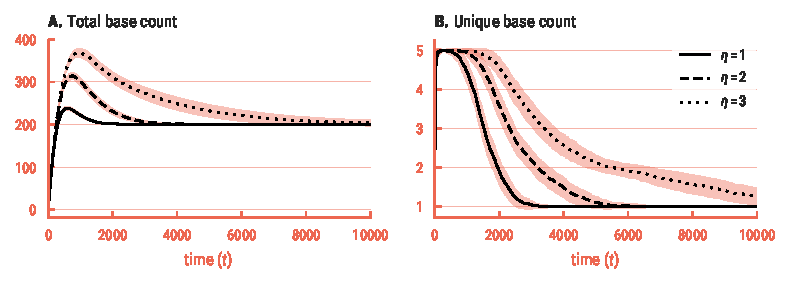
\includegraphics[trim=\figleftmarginA{} 0 0 \figtopmargin]{HUR02-results}	
	\caption{Effects of $\xi$, the parameter regulating the production strategy in the additive base game. Clearly, smaller values lead to slower convergence time.
		\figdetails{
			\figid{HUR02}		
			Results shown for $N=200$, $B=10$; avg.\ of 300 runs; 1 std.\ shaded.}
		\label{fig:app-counting-games:effects-xi}}
\end{SCfigure}
%- - - - - - - -


%- - - - - - - -
\begin{SCfigure}
	% Results HUR01b
	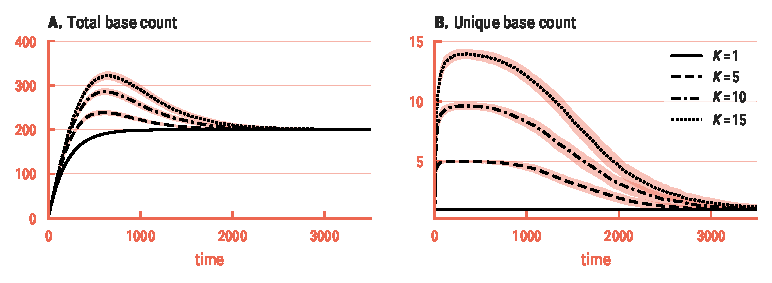
\includegraphics[trim=\figleftmarginA{} 0 0 \figtopmargin]{HUR01-results}	
	\caption{The effect of $K$, the number of bases, in the additive base game. 
		\figdetails{
			\figid{HUR01}
			Results shown for $N=200$, $\xi=1$; avg.\ of 300 runs; 1 std.\ shaded.}
		\label{fig:app-counting-games:effect-B}}
\end{SCfigure}
%- - - - - - - -




%——————————————————————————————————————————————————————————
\paragraph{effects of the number of simple numerals}

How does the number of simple numerals influence the game?
Figure \ref{fig:app-counting-games:effect-B} summarises some experiments of the additive base game with $B \in \{1,10,20,30\}$.
Although these simple experiments do not yield strong conclusions, the convergence time is not strongly influenced by $B$.
That is, certainly not in a power law fashion, like population size.
Rather, the convergence time does not seem to depend on $K$.
One reason for this is that convergence time in the Dirichlet-categorical naming game was also not found to be strongly influenced by $K$.



%——————————————————————————————————————————————————————————
\showbibliography

\end{document}
